\section{位移的物理账本（二）：低空与第三维度}

\subsection{二维锁定、空域秩序成本与举升的物理账本}

位移的代价可以分成两部分。一部分随距离增长，可以通过更好的动力和更高的效率逐步压缩；另一部分由路径的拓扑决定，不随效率改进而改变。当一段位移的地面路径被已经建成的结构固定住时，车辆层面的任何优化都不会缩短它。

\subhead{二维锁定与第三维度}

低空经济的核心不是“飞行器”，而是“第三维度”。地面交通被二维网络锁住。道路、桥梁、隧道、红绿灯、路口、停车场、产权边界、城市密度和地形结构，共同决定了人和货物如何移动。很多时候，A 点到 B 点的直线距离并不远，但现实路径会被河流、山体、拥堵、建筑、道路等级、换乘节点和行政边界拉长。地面交通的黏滞，不只来自距离，而来自路径被拓扑锁定。

低空经济真正有价值的地方，就在于它试图打开第三维度。它不是在地面上再造一条路，而是在某些地面拓扑过重的场景中，绕开道路网络的限制。跨江、跨山、海岛、灾害现场、山区补给、电力巡检、农林植保、消防侦察、医疗急送，这些场景的共同点不是“飞起来很酷”，而是地面路径太重。低空路径如果能够用更短时间、更少连续基础设施、更少地面耦合完成有效位移，它就有真实价值。

因此，\key{低空经济的第一性问题不是能不能飞，而是值不值得飞。}一架飞行器从地面升空，并不自动意味着效率提高。飞行会引入新的成本：飞行器制造、能耗、维护、安全冗余、起降点、噪声、气象、通信、监管、保险和事故责任。如果地面路径已经足够低成本，低空方案只是把一个简单任务变成高成本表演。只有当地面位移的总作用量足够高，低空路径才可能成为更优解。所谓总作用量，不是狭义物理公式，而是一次位移背后的全部代价：时间、能量、设备、基础设施、维护、风险、等待、监管、噪声、责任和系统韧性。低空经济能否成立，取决于它是否真正降低单位有效位移的总代价。

这里必须先澄清一个常见误解：低空经济不等于电动 eVTOL，也不等于无人机。燃油小型飞机、直升机、通用航空固定翼、农林作业飞机、医疗救援直升机、低空观光飞行器，都属于广义低空经济。电动化是低空经济的重要方向，但不是低空经济的全部。把低空经济窄化成“电动飞行汽车”，会遮蔽它真正的产业结构：它首先是低空位移、低空作业和低空服务的体系，而不是某一种动力形式的胜利。把它还原为一个位移系统之后，它的结构优势才可以被准确描述。

\subhead{空域秩序成本}

低空的优势，是减少对连续道路基础设施的依赖。地面交通要铺路、架桥、挖隧道、修停车场，还要处理路口、拥堵、产权和城市空间。低空路径中间不需要铺设实体道路，不需要为每一米路径浇筑基础设施。这是它相对于地面交通的结构优势：它用空间自由度，换取路径压缩。但这不是免费自由。低空只是少修了道路，不是少付了代价。它把黏滞从道路重资产，转移到空域治理、安全验证、起降接口、通信导航、气象感知、噪声管理、责任追踪和高频运营之中。少量无人机飞起来不难，难的是让大量飞行器在城市和产业空间中长期、安全、低成本、可监管、可追责地运行。

这就是低空经济的基本悖论：它打开了第三维度，也制造了第三维度的秩序成本。地面交通的秩序由道路显性规定。车道、红绿灯、路口、限速、标线、护栏和停车位，构成了可见的交通语法。低空交通没有这些天然边界。空中路径看似自由，但一旦飞行器密集运行，就必须重新定义航线、高度、间隔、避障、应急降落、禁飞区、噪声边界、通信协议、身份识别和事故责任。没有这套秩序，低空不是自由空间，而是高风险空间。

所以，低空经济真正的基础设施，不只是起降点和飞行器，而是低空操作系统。它包括空域划分、航线审批、实时监控、动态避障、气象数据、通信链路、飞行日志、身份识别、维护标准、保险机制、事故处理和责任归属。飞行器是可见部分，空域秩序才是底层结构。

空域秩序可以逐层设计，飞行本身的物理约束不能。从 RTG 角度看，低空经济并不低黏滞。它的资源势垒首先来自飞行本身。飞行器比地面车辆更怕重量。地面车辆重一点，主要是能耗和磨损增加；飞行器重一点，直接压缩载荷、航程和安全边界。机体材料、动力冗余、通信设备、感知系统、维护体系，都进入物理账本。低空经济看起来绕开了道路重资产，但没有绕开质量、能量和安全冗余。

\subhead{举升的物理账本}

资源势垒中最难绕过的一项落在储能上。当前电动低空飞行器最硬的瓶颈，就是电池。对地面车辆来说，电池笨重主要表现为车重增加、能耗上升、成本变高；但对飞行器来说，重量不是线性负担，而是直接决定能不能飞、飞多远、载多少、留多少安全冗余。汽车可以用更大的电池换更长续航，代价是更重、更贵；低空飞行器却不能简单这样做，因为更大的电池本身也要被举起来。电池增加航程的同时也增加自重，新增能量的一部分会被用来搬运电池自己。这使电动低空飞行器很容易陷入一个物理悖论：想飞得更远，就要带更多电池；带更多电池，又会压缩载荷和航程收益。

这个悖论可以从悬停所需的功率上看清楚。按动量理论，旋翼把空气向下加速以获得升力，所需机械功率为
\begin{equation}
P_{\text{悬停}}=\sqrt{\frac{(mg)^3}{2\rho A}}
\label{eq:ch26-hover}
\end{equation}
前式是理想桨盘动量理论给出的诱导功率，$m$为总质量，$\rho$为空气密度，$A$为模型下的有效桨盘面积。固定$A$和$\rho$时，质量翻倍，理想诱导功率增至约2.83倍。实际电功率还要计入型阻、非理想流动、传动效率与辅助设备；多旋翼的相互作用也要另计。

把储能与功率相除，续航与质量的关系可以直接写出，

\begin{equation}
t_{\text{悬停}}\approx\frac{\epsilon e_bm_b\sqrt{2\rho A}}{g^{3/2}(m_0+m_b)^{3/2}}
\end{equation}

$m_0$为固定的非电池质量，$m_b$为电池质量，$e_b$为可用比能量，$\epsilon$为综合效率。固定桨盘面积与效率，增加电池在早期会延长悬停时间；继续增加时，自重的功率支出逐渐占优。这个简化模型的极值在$m_b=2m_0$，不是实际设计推荐值。只有在储能与总质量成正比的另一组假设下，才得到$m^{-1/2}$的尺度关系；“新增质量都是电池”本身不足以推出它。巡航还须另建任务模型。

地面滚动与旋翼悬停具有不同能量结构。悬停高度不变，机体的重力势能并未持续增加；功率主要用于向空气传递动量，并支付非理想流动、阻力与设备损耗。固定翼巡航又有自己的升阻与任务条件。比较电动车与飞行器，应采用完整飞行剖面、包级储能、载荷和备用能量。

燃油小型飞机和直升机在低空经济中不会马上被电动化完全替代。航空煤油的质量能量密度约为 43 兆焦每千克，比当前锂离子电池高出数十倍\cite{viswanathan2022challenges}，这一优势在航程、载荷、应急、偏远地区和高强度作业中尤其明显。燃油飞行器的问题不在于它不能飞，而在于噪声、排放、维护、成本、安全、飞行员依赖和运行门槛。电动飞行器的问题则相反：它在控制、维护、噪声和平台化上有优势，但受制于电池自重、续航、载荷和安全冗余。二者不是简单先进与落后的关系，而是在不同约束下的不同解。

低空经济的动力路线，很可能不是单一替代，而是场景分化。短途、低载荷、固定航线、城市周边、低噪声敏感场景，适合电动化；长航程、高载荷、偏远地区、应急救援、专业作业，燃油或混合动力仍可能长期存在。真正的问题不是“电动还是燃油”，而是不同位移任务需要什么样的能量密度、功率密度、维护体系和安全冗余。能量与载荷的账算完之后，剩下的两项约束不来自飞行器本身，而来自系统必须被社会接受的方式。

\begin{figure}[ht]
\centering
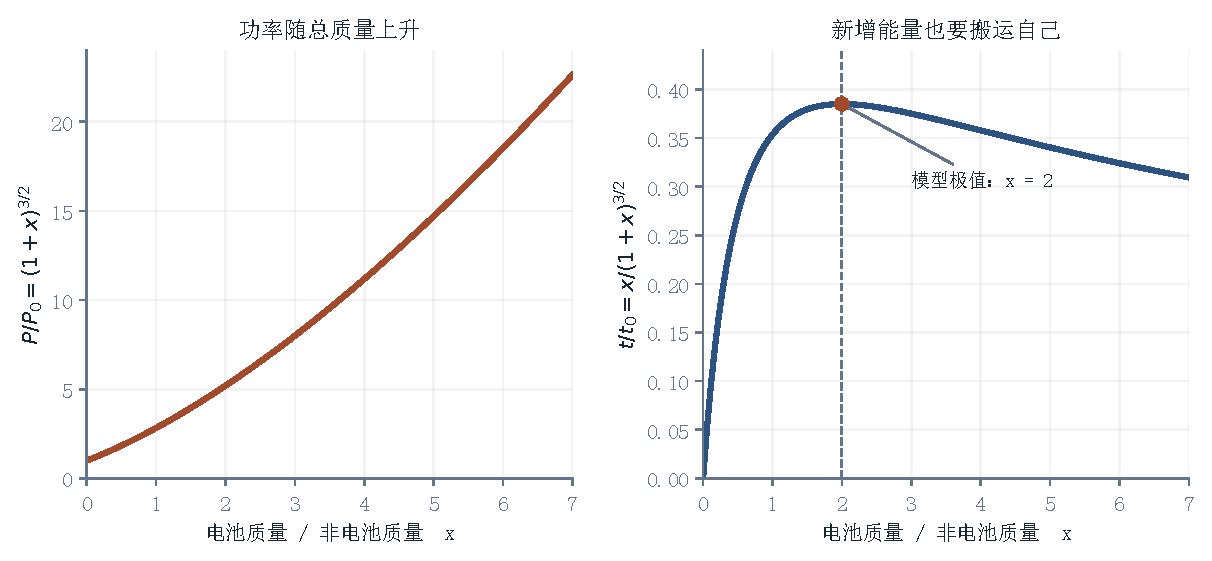
\includegraphics[width=\textwidth]{figures/hover-tradeoff.pdf}
\caption{固定桨盘面积、空气密度与效率的理想悬停模型。$x=m_b/m_0$；$P_0$为非电池质量对应的诱导功率，$t_0=\epsilon e_bm_0/P_0$。归一化续航在$x=2$达到极值。实际设计还要计入结构、功率限制与任务剖面。}
\label{fig:lift-ledger}
\end{figure}



\subsection{验证时间、场景匹配与治理层的产业价值}

\subhead{验证时间与空域耦合}

低空经济的时间刚性来自验证。它不能靠几次试飞证明成熟。飞行是高后果系统，需要飞行小时、适航认证、维护规程、事故统计、公众接受和监管信任。越接近载人、城市密集区和高频运营，验证越慢，责任越重。飞行器可以很快发布概念机，低空位移系统却不能很快获得社会信任。

飞行能力、设计符合性、单机状态和运营许可是不同层次。Joby在2026年3月宣布首架用于TIA的FAA符合性飞机开始飞行测试；9月另行公布的J208自主飞行巡展，则使用改装的Cessna Caravan与受监督运行。\cite{joby2026conforming,joby2026j208} 两项进展属于不同平台，不能合并为“自主电动空中出租车已完成全部商业准入”。FAA与EASA的框架也分别处理设计和运行要求。\cite{faa2026aam,easa2026vtol}

它的拓扑耦合来自空域。低空不是空白空间，而是城市、机场、军航、民航、公安、消防、建筑、通信、气象、隐私、噪声和公众安全共同交织的空间。飞行器越多，系统越不是“单机飞行”，而是“空域网络”。空中一旦高密度运行，风险就不再来自单个飞行器，而来自整个空域系统的协调能力。因此，低空经济不是轻资产经济，而是轻道路、重治理的位移系统。它省掉了一部分地面连续基础设施，却增加了大量空域规则、通信接口、验证体系和责任结构。它不是无摩擦未来，而是另一种黏滞分布。这也决定了它的落地顺序。

低空经济最先成熟的，不会是大众空中通勤，而是高价值、强约束、可验证的任务。电力巡检、管线巡查、农林植保、消防侦察、灾害勘察、医疗物资急送、海岛补给、山地物流、港口园区、矿区、景区、固定线路接驳，这些场景更接近低空经济的真实入口。它们运行域相对清晰，地面替代路径很重，责任边界较容易定义，运营数据可以逐步积累。反过来，大众空中通勤是最难的场景。它要求低噪声、高安全、低价格、高准点、高密度、低等待、高冗余、公众信任和监管协同同时成立。这不是造出几架 eVTOL 就能解决的问题。城市空中出租车可以出现，但它更可能先是高价、固定航线、少数场景的服务，而不是像公交、地铁、网约车那样覆盖日常生活。落地顺序由约束决定，不由愿望决定。

\subhead{场景匹配}

落地顺序确定之后，筛选标准也就清楚了。低空经济真正要避免的，不是“飞不起来”，而是场景错配。如果它用于地面拓扑过重的地方，就是有效旁路；如果用于普通地面出行，就是高成本炫技。它如果服务应急、巡检、农业、山区、海岛、消防、医疗和固定走廊，就可能降低总作用量；如果只是为了让城市中产从一个商圈飞到另一个商圈，可能只是把道路拥堵换成空域监管、噪声投诉、高保险成本和低利用率设备。因此，判断低空经济，不应先问“市场有多大”，而应先问“哪些位移值得飞”。不是所有位移都值得三维化。低空路径的价值，取决于地面路径有多重、时间价值有多高、任务风险有多大、运行域有多清晰、责任链有多完整。一个成熟产业不会把所有需求都往天上搬，而是筛选那些地面黏滞足够高、低空替代足够有优势的场景。

这也意味着，低空经济很难成为“空中私家车”。私人飞行器的利用率、安全责任、维护成本、起降接口、空域审批和事故风险，都比私家车更难社会化。真正可能成熟的形态，仍然是运营化：固定任务、固定航线、固定空域、固定维护、固定责任链。低空飞行器不是被个人占有才产生价值，而是在高频、可控、可维护的任务网络中产生价值。这一点和自动驾驶运营车相似。自动驾驶运营车的关键，不是让每个人拥有一辆无人私家车，而是用高利用率运营车辆覆盖大量日常位移；低空经济的关键，也不是让每个人拥有一架低空飞行器，而是让飞行器在高价值场景中形成稳定运营网络。

二者的差别在于：自动驾驶运营车更可能覆盖大众日常出行，低空经济更适合补足地面位移过重的特殊场景。前者重构日常交通，后者打开高黏滞场景的旁路。场景分工确定之后，产业价值沉淀的位置也就确定了。

\subhead{治理层的产业价值}

低空经济的产业价值，不会只沉淀在机体制造上。飞行器当然重要，但更重要的是空域管理系统、通信导航、起降接口、维修体系、飞行数据平台、气象服务、保险定价、适航认证、运营组织、应急处置和城市治理接口。卖飞行器只是第一层，运营低空秩序才是更深层。如果每个地方各建一套低空平台，各搞一套标准，各自招商造景，低空经济就会从第三维度的打开，变成新的碎片化工程。真正成熟的低空产业，需要统一规则、互认标准、跨区域航线、事故责任、数据接口和监管平台。否则，飞行器能飞，产业却不能规模化运行。

市场预测反映需求预期，项目收入来自实际可服务的任务。起降接口、许可、噪声约束、天气可用率与周转时间，会把总需求筛成能够经营的线路。治理层的产业价值就在这里：把一段理论可飞的路径，组织成可验证、可维护并能持续兑现的服务。

低空经济最好的状态，是成为位移系统的补充层，而不是新的万能叙事。它不应被赋予替代地面交通的使命，也不该被贬低为纯粹概念泡沫。它有真实价值，但价值来自场景匹配。它的第一原则很简单：当地面路径太重，低空路径才有意义；当飞行的治理成本低于地面绕行成本，低空经济才成立。所以，低空经济的判断标准不是飞行器能飞多远、飞多快，而是三个问题：第一，这个任务的地面位移是否足够高黏滞；第二，低空路径是否能降低单位有效位移的总代价；第三，这个低空系统是否可验证、可监管、可追责、可持续运营。答不上这三个问题，所谓低空经济就只是飞行器展示、地方口号和资本故事。答得上，它才是新的位移层。

把这条第一原则写成不等式，

\begin{equation}
A_{\text{低空}}+A_{\text{治理}}<A_{\text{地面绕行}}
\end{equation}

式中 $A_{\text{地面绕行}}$ 是完成同一次位移走地面路径所支付的总作用量；$A_{\text{低空}}$ 是低空路径自身的作用量，包含飞行器制造与折旧、能耗、维护、安全冗余和起降点；$A_{\text{治理}}$ 是第三维度的秩序成本，包含空域划分、航线审批、实时监控、通信导航、气象感知、适航验证、保险与责任结构。三项必须先折算到同一口径，并分摊到同一次有效位移上（时间、能量、风险、占地、责任），单位随口径而定，因此这是一个判定条件，而不是可以直接相加的实测量。它的含义是：低空路径的价值不由它省下了多少道路决定，而由它省下的地面代价是否大于它自己带来的总代价决定。适用边界在折算：哪些成本能进入同一个账本取决于任务本身，同一组飞行器在电力巡检或医疗急送上可能满足这个不等式，在城市商圈之间的日常通勤上可能不满足，这正是“场景匹配”的准确含义；制度合法性、公共接受与长期信任难以折算时，不等式只覆盖可折算的部分。

低空经济的本质，不是把交通搬到天上。它是在地面拓扑过重的地方打开第三维度，又在第三维度中重新支付能量、载荷、安全、监管、责任和运营代价。它的价值不在于天空看起来无限，而在于少数场景中，天空确实比地面更低黏滞。它的边界也在这里：低空不是无摩擦未来，而是一种高治理成本下的位移旁路。
